% Created 2017-03-03 Fri 08:15
\documentclass[11pt]{article}
\usepackage[utf8]{inputenc}
\usepackage[T1]{fontenc}
\usepackage{fixltx2e}
\usepackage{graphicx}
\usepackage{longtable}
\usepackage{float}
\usepackage{wrapfig}
\usepackage{rotating}
\usepackage[normalem]{ulem}
\usepackage{amsmath}
\usepackage{textcomp}
\usepackage{marvosym}
\usepackage{wasysym}
\usepackage{amssymb}
\usepackage{hyperref}
\tolerance=1000
\date{Feb 27-Mar 3, 2017}
\title{Week 7 lecture notes - PSYC 3435}
\hypersetup{
  pdfkeywords={},
  pdfsubject={},
  pdfcreator={Emacs 25.1.1 (Org mode 8.2.10)}}
\begin{document}

\maketitle

\section*{Sampling}
\label{sec-1}

Definitions:
\begin{itemize}
\item Population: everybody that the research tries to make conclusions about
\item Sample: the subset of the population that actually participates in the research
\end{itemize}

Goals of sampling:
\begin{itemize}
\item maximize representativeness (how closely sample matches population)
\item reduce bias (systematic difference between sample and population)
\end{itemize}

\subsection*{Sampling methods}
\label{sec-1-1}
Type 1: Probability sampling - individuals chosen at random in such a way that we know the probability that any one individual is selected

Examples:
\begin{itemize}
\item simple random sample - each individual has an \textbf{equal} chance of being selected
\item cluster sample - population divided into groups (clusters). Group(s) selected randomly, then individuals chosen randomly from each cluster
\item stratified random sample - sample chosen so that proportion of individuals with a particular characteristic is equivalent in population and sample
\item systematic sample - pick a random starting number, then choose every k-th person after that.
\end{itemize}

Type 2: Convenience sampling - individuals chosen non-randomly

Examples: 
\begin{itemize}
\item Convenience sampling -- use participants who are easy to get (volunteers, etc.)
\item Quota sampling - identify specific subgroups, then take from each group until desired number of individuals
\end{itemize}

\section*{Experimental Control}
\label{sec-2}

When we do an experiment, we see variability in the DV.  How much of this variability is due to our experimental manipulation?

Let's do a little math:

$T = NR_{exp} + NR_{other} + R$, where
\begin{itemize}
\item $T$ = total variability in DV
\item $NR_{exp}$ = non-random variability due to IV manipulation
\item $NR_{other}$ = non-random extraneous variables that covary with IV (confounds)
\item $R$ = random variability due to measurement error
\end{itemize}

Our goal is to detect $NR_{exp}$, so we need to \emph{minimize} $NR_{other}$ and $R$

Visualization:

Imagine the difference sources of variability as weights:

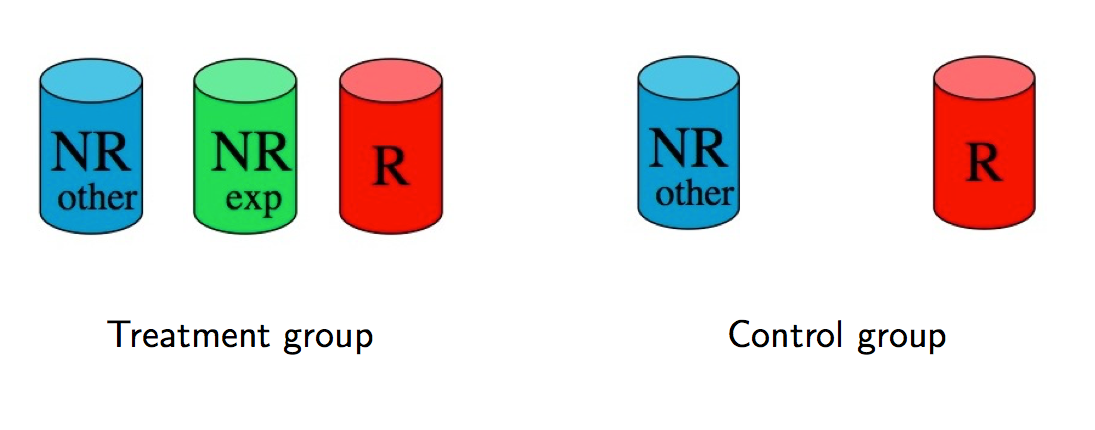
\includegraphics[width=.9\linewidth]{figures/weights.png}

If $NR_{other}$ and $R$ are \emph{large} relative to $NR_{exp}$, then detecting the difference may be difficult

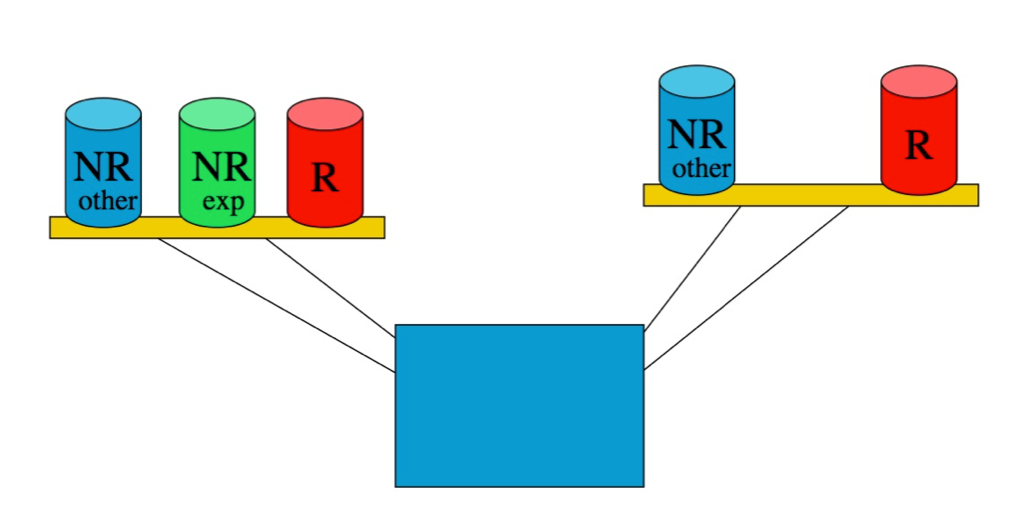
\includegraphics[width=.9\linewidth]{figures/balance1.png}

But if we reduce the size of $NR_{other}$ and $R$ relative to $R_{exp}$, detecting the difference becomes much easier.

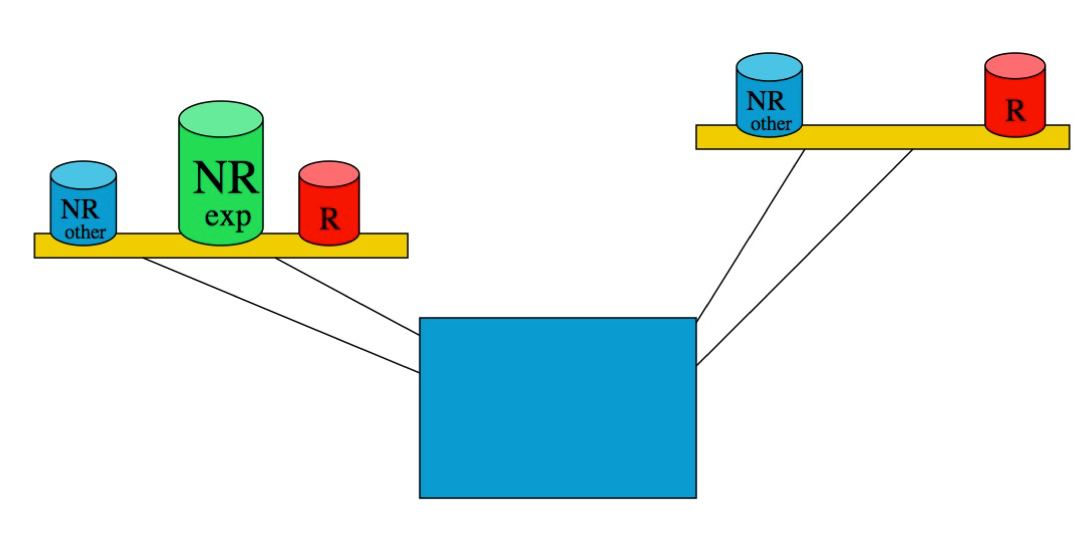
\includegraphics[width=.9\linewidth]{figures/balance2.png}
% Emacs 25.1.1 (Org mode 8.2.10)
\end{document}